\documentclass{article}
\usepackage{pgfplots}
\pgfplotsset{compat=newest}

\pagestyle{empty}

\begin{document}
In this note we explore the problem of the average value 
of the length of the longest increasing subsequence in 
a randomly generated sequence of a given length.

\section{Problem statement}
The {\it longest increasing subsequence} of a given sequence
is a subsequence - i.e. elements are chosen in the same order 
as they appear in the given sequence -- that is sorted. The problem 
is to find the longest among such subsequences.

An interesting question is -- given a randomly generated sequence
what is the average length of longest increasing subsequence.

\section{Experiment setup}
To generate a sequence of length $N$ each element is independently generated
using uniform distribution of integers in the range $[0,10\times N]$. For each
$N$ we performed $200$ experiments. The blue graph below shows the average
value of the longest increasing subsequence plus-minus standard deviation. The
red graph shows function $2\sqrt{x}$ which grows almost at the same rate, supporting 
the hypothesis that average length of the longest increasing subsequence of size $N$
is $O(\sqrt{N})$.


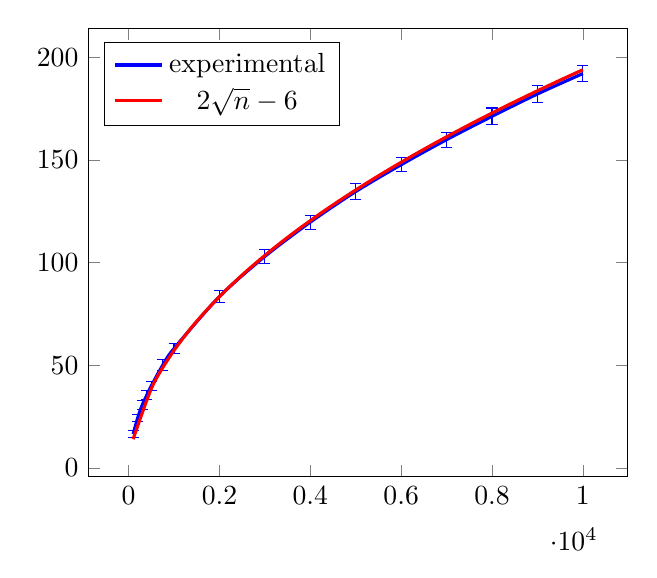
\begin{tikzpicture}
\begin{axis}[legend pos=north west]
\addplot+[line width=0.4mm,smooth,mark=,error bars/.cd, y dir=both,y explicit ]
    coordinates {
        (100, 16.535) +- (1.70551311926939,1.70551311926939)
        (200, 24.415) +- (1.75862872716216,1.75862872716216)
        (300, 30.665) +- (2.31360649203792,2.31360649203792)
        (400, 35.435) +- (2.22615700254946,2.22615700254946)
        (500, 40.005) +- (2.31192019758468,2.31192019758468)
        (750, 50.02) +- (2.62099217854613,2.62099217854613)
        (1000, 58.19) +- (2.30518979695816,2.30518979695816)
        (2000, 83.485) +- (2.88786685981193,2.88786685981193)
        (3000, 103.05) +- (3.247691487811,3.247691487811)
        (4000, 119.75) +- (3.45217322856197,3.45217322856197)
        (5000, 134.665) +- (3.72730130255122,3.72730130255122)
        (6000, 147.74) +- (3.43691722332674,3.43691722332674)
        (7000, 159.945) +- (3.66087079804792,3.66087079804792)
        (8000, 171.305) +- (4.04870040877316,4.04870040877316)
        (9000, 182.195) +- (4.11180921250001,4.11180921250001)
        (10000, 192.155) +- (3.88213536600671,3.88213536600671)
    };
\addlegendentryexpanded{experimental}
\addplot+[line width=0.4mm,smooth,mark=,domain=100:10000] {2*sqrt(x)-6};
\addlegendentryexpanded{$2\sqrt{n}-6$}
\end{axis}
\end{tikzpicture}

Dmitri Volper 
\end{document}
